% Options for packages loaded elsewhere
% Options for packages loaded elsewhere
\PassOptionsToPackage{unicode}{hyperref}
\PassOptionsToPackage{hyphens}{url}
\PassOptionsToPackage{dvipsnames,svgnames,x11names}{xcolor}
%
\documentclass[
  spanish,
  11pt,
]{article}
\usepackage{xcolor}
\usepackage[margin=2.5cm]{geometry}
\usepackage{amsmath,amssymb}
\setcounter{secnumdepth}{5}
\usepackage{iftex}
\ifPDFTeX
  \usepackage[T1]{fontenc}
  \usepackage[utf8]{inputenc}
  \usepackage{textcomp} % provide euro and other symbols
\else % if luatex or xetex
  \usepackage{unicode-math} % this also loads fontspec
  \defaultfontfeatures{Scale=MatchLowercase}
  \defaultfontfeatures[\rmfamily]{Ligatures=TeX,Scale=1}
\fi
\usepackage{lmodern}
\ifPDFTeX\else
  % xetex/luatex font selection
\fi
% Use upquote if available, for straight quotes in verbatim environments
\IfFileExists{upquote.sty}{\usepackage{upquote}}{}
\IfFileExists{microtype.sty}{% use microtype if available
  \usepackage[]{microtype}
  \UseMicrotypeSet[protrusion]{basicmath} % disable protrusion for tt fonts
}{}
\usepackage{setspace}
\makeatletter
\@ifundefined{KOMAClassName}{% if non-KOMA class
  \IfFileExists{parskip.sty}{%
    \usepackage{parskip}
  }{% else
    \setlength{\parindent}{0pt}
    \setlength{\parskip}{6pt plus 2pt minus 1pt}}
}{% if KOMA class
  \KOMAoptions{parskip=half}}
\makeatother
% Make \paragraph and \subparagraph free-standing
\makeatletter
\ifx\paragraph\undefined\else
  \let\oldparagraph\paragraph
  \renewcommand{\paragraph}{
    \@ifstar
      \xxxParagraphStar
      \xxxParagraphNoStar
  }
  \newcommand{\xxxParagraphStar}[1]{\oldparagraph*{#1}\mbox{}}
  \newcommand{\xxxParagraphNoStar}[1]{\oldparagraph{#1}\mbox{}}
\fi
\ifx\subparagraph\undefined\else
  \let\oldsubparagraph\subparagraph
  \renewcommand{\subparagraph}{
    \@ifstar
      \xxxSubParagraphStar
      \xxxSubParagraphNoStar
  }
  \newcommand{\xxxSubParagraphStar}[1]{\oldsubparagraph*{#1}\mbox{}}
  \newcommand{\xxxSubParagraphNoStar}[1]{\oldsubparagraph{#1}\mbox{}}
\fi
\makeatother

\usepackage{color}
\usepackage{fancyvrb}
\newcommand{\VerbBar}{|}
\newcommand{\VERB}{\Verb[commandchars=\\\{\}]}
\DefineVerbatimEnvironment{Highlighting}{Verbatim}{commandchars=\\\{\}}
% Add ',fontsize=\small' for more characters per line
\usepackage{framed}
\definecolor{shadecolor}{RGB}{241,243,245}
\newenvironment{Shaded}{\begin{snugshade}}{\end{snugshade}}
\newcommand{\AlertTok}[1]{\textcolor[rgb]{0.68,0.00,0.00}{#1}}
\newcommand{\AnnotationTok}[1]{\textcolor[rgb]{0.37,0.37,0.37}{#1}}
\newcommand{\AttributeTok}[1]{\textcolor[rgb]{0.40,0.45,0.13}{#1}}
\newcommand{\BaseNTok}[1]{\textcolor[rgb]{0.68,0.00,0.00}{#1}}
\newcommand{\BuiltInTok}[1]{\textcolor[rgb]{0.00,0.23,0.31}{#1}}
\newcommand{\CharTok}[1]{\textcolor[rgb]{0.13,0.47,0.30}{#1}}
\newcommand{\CommentTok}[1]{\textcolor[rgb]{0.37,0.37,0.37}{#1}}
\newcommand{\CommentVarTok}[1]{\textcolor[rgb]{0.37,0.37,0.37}{\textit{#1}}}
\newcommand{\ConstantTok}[1]{\textcolor[rgb]{0.56,0.35,0.01}{#1}}
\newcommand{\ControlFlowTok}[1]{\textcolor[rgb]{0.00,0.23,0.31}{\textbf{#1}}}
\newcommand{\DataTypeTok}[1]{\textcolor[rgb]{0.68,0.00,0.00}{#1}}
\newcommand{\DecValTok}[1]{\textcolor[rgb]{0.68,0.00,0.00}{#1}}
\newcommand{\DocumentationTok}[1]{\textcolor[rgb]{0.37,0.37,0.37}{\textit{#1}}}
\newcommand{\ErrorTok}[1]{\textcolor[rgb]{0.68,0.00,0.00}{#1}}
\newcommand{\ExtensionTok}[1]{\textcolor[rgb]{0.00,0.23,0.31}{#1}}
\newcommand{\FloatTok}[1]{\textcolor[rgb]{0.68,0.00,0.00}{#1}}
\newcommand{\FunctionTok}[1]{\textcolor[rgb]{0.28,0.35,0.67}{#1}}
\newcommand{\ImportTok}[1]{\textcolor[rgb]{0.00,0.46,0.62}{#1}}
\newcommand{\InformationTok}[1]{\textcolor[rgb]{0.37,0.37,0.37}{#1}}
\newcommand{\KeywordTok}[1]{\textcolor[rgb]{0.00,0.23,0.31}{\textbf{#1}}}
\newcommand{\NormalTok}[1]{\textcolor[rgb]{0.00,0.23,0.31}{#1}}
\newcommand{\OperatorTok}[1]{\textcolor[rgb]{0.37,0.37,0.37}{#1}}
\newcommand{\OtherTok}[1]{\textcolor[rgb]{0.00,0.23,0.31}{#1}}
\newcommand{\PreprocessorTok}[1]{\textcolor[rgb]{0.68,0.00,0.00}{#1}}
\newcommand{\RegionMarkerTok}[1]{\textcolor[rgb]{0.00,0.23,0.31}{#1}}
\newcommand{\SpecialCharTok}[1]{\textcolor[rgb]{0.37,0.37,0.37}{#1}}
\newcommand{\SpecialStringTok}[1]{\textcolor[rgb]{0.13,0.47,0.30}{#1}}
\newcommand{\StringTok}[1]{\textcolor[rgb]{0.13,0.47,0.30}{#1}}
\newcommand{\VariableTok}[1]{\textcolor[rgb]{0.07,0.07,0.07}{#1}}
\newcommand{\VerbatimStringTok}[1]{\textcolor[rgb]{0.13,0.47,0.30}{#1}}
\newcommand{\WarningTok}[1]{\textcolor[rgb]{0.37,0.37,0.37}{\textit{#1}}}

\usepackage{longtable,booktabs,array}
\usepackage{calc} % for calculating minipage widths
% Correct order of tables after \paragraph or \subparagraph
\usepackage{etoolbox}
\makeatletter
\patchcmd\longtable{\par}{\if@noskipsec\mbox{}\fi\par}{}{}
\makeatother
% Allow footnotes in longtable head/foot
\IfFileExists{footnotehyper.sty}{\usepackage{footnotehyper}}{\usepackage{footnote}}
\makesavenoteenv{longtable}
\usepackage{graphicx}
\makeatletter
\newsavebox\pandoc@box
\newcommand*\pandocbounded[1]{% scales image to fit in text height/width
  \sbox\pandoc@box{#1}%
  \Gscale@div\@tempa{\textheight}{\dimexpr\ht\pandoc@box+\dp\pandoc@box\relax}%
  \Gscale@div\@tempb{\linewidth}{\wd\pandoc@box}%
  \ifdim\@tempb\p@<\@tempa\p@\let\@tempa\@tempb\fi% select the smaller of both
  \ifdim\@tempa\p@<\p@\scalebox{\@tempa}{\usebox\pandoc@box}%
  \else\usebox{\pandoc@box}%
  \fi%
}
% Set default figure placement to htbp
\def\fps@figure{htbp}
\makeatother


% definitions for citeproc citations
\NewDocumentCommand\citeproctext{}{}
\NewDocumentCommand\citeproc{mm}{%
  \begingroup\def\citeproctext{#2}\cite{#1}\endgroup}
\makeatletter
 % allow citations to break across lines
 \let\@cite@ofmt\@firstofone
 % avoid brackets around text for \cite:
 \def\@biblabel#1{}
 \def\@cite#1#2{{#1\if@tempswa , #2\fi}}
\makeatother
\newlength{\cslhangindent}
\setlength{\cslhangindent}{1.5em}
\newlength{\csllabelwidth}
\setlength{\csllabelwidth}{3em}
\newenvironment{CSLReferences}[2] % #1 hanging-indent, #2 entry-spacing
 {\begin{list}{}{%
  \setlength{\itemindent}{0pt}
  \setlength{\leftmargin}{0pt}
  \setlength{\parsep}{0pt}
  % turn on hanging indent if param 1 is 1
  \ifodd #1
   \setlength{\leftmargin}{\cslhangindent}
   \setlength{\itemindent}{-1\cslhangindent}
  \fi
  % set entry spacing
  \setlength{\itemsep}{#2\baselineskip}}}
 {\end{list}}
\usepackage{calc}
\newcommand{\CSLBlock}[1]{\hfill\break\parbox[t]{\linewidth}{\strut\ignorespaces#1\strut}}
\newcommand{\CSLLeftMargin}[1]{\parbox[t]{\csllabelwidth}{\strut#1\strut}}
\newcommand{\CSLRightInline}[1]{\parbox[t]{\linewidth - \csllabelwidth}{\strut#1\strut}}
\newcommand{\CSLIndent}[1]{\hspace{\cslhangindent}#1}

\ifLuaTeX
\usepackage[bidi=basic]{babel}
\else
\usepackage[bidi=default]{babel}
\fi
% get rid of language-specific shorthands (see #6817):
\let\LanguageShortHands\languageshorthands
\def\languageshorthands#1{}


\setlength{\emergencystretch}{3em} % prevent overfull lines

\providecommand{\tightlist}{%
  \setlength{\itemsep}{0pt}\setlength{\parskip}{0pt}}



 


\usepackage{microtype}
\usepackage{float}
\usepackage{booktabs}
\usepackage{graphicx}
\usepackage{amsmath, amssymb}
\usepackage{caption}
\captionsetup[figure]{labelfont=bf, labelsep=period}
\usepackage{csquotes}
\usepackage{hyperref}
\makeatletter
\@ifpackageloaded{caption}{}{\usepackage{caption}}
\AtBeginDocument{%
\ifdefined\contentsname
  \renewcommand*\contentsname{Tabla de contenidos}
\else
  \newcommand\contentsname{Tabla de contenidos}
\fi
\ifdefined\listfigurename
  \renewcommand*\listfigurename{Listado de Figuras}
\else
  \newcommand\listfigurename{Listado de Figuras}
\fi
\ifdefined\listtablename
  \renewcommand*\listtablename{Listado de Tablas}
\else
  \newcommand\listtablename{Listado de Tablas}
\fi
\ifdefined\figurename
  \renewcommand*\figurename{Figura}
\else
  \newcommand\figurename{Figura}
\fi
\ifdefined\tablename
  \renewcommand*\tablename{Tabla}
\else
  \newcommand\tablename{Tabla}
\fi
}
\@ifpackageloaded{float}{}{\usepackage{float}}
\floatstyle{ruled}
\@ifundefined{c@chapter}{\newfloat{codelisting}{h}{lop}}{\newfloat{codelisting}{h}{lop}[chapter]}
\floatname{codelisting}{Listado}
\newcommand*\listoflistings{\listof{codelisting}{Listado de Listados}}
\makeatother
\makeatletter
\makeatother
\makeatletter
\@ifpackageloaded{caption}{}{\usepackage{caption}}
\@ifpackageloaded{subcaption}{}{\usepackage{subcaption}}
\makeatother
\usepackage{bookmark}
\IfFileExists{xurl.sty}{\usepackage{xurl}}{} % add URL line breaks if available
\urlstyle{same}
\hypersetup{
  pdftitle={Métodos de Bootstrapping: Fundamentos y Aplicaciones},
  pdfauthor={David Valcárcel},
  pdflang={es},
  colorlinks=true,
  linkcolor={MidnightBlue},
  filecolor={Maroon},
  citecolor={MidnightBlue},
  urlcolor={MidnightBlue},
  pdfcreator={LaTeX via pandoc}}


\title{Métodos de Bootstrapping: Fundamentos y Aplicaciones}
\author{David Valcárcel}
\date{2025-07-17}
\begin{document}
\maketitle

\renewcommand*\contentsname{Tabla de contenidos}
{
\hypersetup{linkcolor=}
\setcounter{tocdepth}{3}
\tableofcontents
}

\setstretch{1.3}
\section{Introducción}\label{introducciuxf3n}

\begin{itemize}
\tightlist
\item
  El \textbf{bootstrapping} es un método de remuestreo propuesto por
  Efron (1979).
\item
  Su objetivo es aproximar la distribución de un estimador estadístico
  utilizando remuestras de los datos observados.
\item
  Se utiliza para construir \textbf{intervalos de confianza}, realizar
  \textbf{contrastes de hipótesis}, y estimar la \textbf{precisión} de
  estadísticas complejas.
\end{itemize}

\begin{center}\rule{0.5\linewidth}{0.5pt}\end{center}

\section{Fundamento teórico}\label{fundamento-teuxf3rico}

\begin{itemize}
\tightlist
\item
  Sea \(\hat{\theta} = s(\mathbf{X})\) un estimador basado en la muestra
  \(\mathbf{X} = (X_1, \dots, X_n)\).
\item
  El problema: no conocemos la distribución de \(\hat{\theta}\).
\item
  Solución: estimarla mediante remuestreo de los datos.
\end{itemize}

\textbf{Principio del bootstrapping}: \textgreater{} La muestra
observada es representativa de la población → simular nuevas muestras
``como si'' provinieran de ella.

\begin{center}\rule{0.5\linewidth}{0.5pt}\end{center}

\section{Bootstrapping no
paramétrico}\label{bootstrapping-no-paramuxe9trico}

\subsection{Fundamentos conceptuales}\label{fundamentos-conceptuales}

El bootstrapping no paramétrico es un método de remuestreo que permite
estimar propiedades de distribuciones (sesgo, error estándar, intervalos
de confianza) \textbf{sin asumir una forma paramétrica subyacente}. Se
basa en el principio de que la muestra observada es la mejor
representación disponible de la población subyacente.

\textbf{Supuesto clave}: Las observaciones son independientes e
idénticamente distribuidas (i.i.d.)

\subsection{Procedimiento ampliado}\label{procedimiento-ampliado}

\subsubsection{1. Muestra bootstrap}\label{muestra-bootstrap}

Dada una muestra original \(\mathbf{X} = (X_1, X_2, \dots, X_n)\): - Se
genera \(\mathbf{X}^{*}\) mediante muestreo con reemplazo - Cada
\(X_i^{*}\) se selecciona independientemente de \(\mathbf{X}\) - Tamaño
de \(\mathbf{X}^{*}\) = tamaño de \(\mathbf{X}\) (\(n\) observaciones) -
\textbf{Propiedad clave}: En promedio, el 63.2\% de los datos originales
aparecen en cada muestra bootstrap
(\(1 - (1 - 1/n)^n \approx 1-e^{-1}\))

\subsubsection{2. Cálculo del
estadístico}\label{cuxe1lculo-del-estaduxedstico}

\begin{itemize}
\tightlist
\item
  \(\hat{\theta}^{*} = s(\mathbf{X}^{*})\) es la versión bootstrap del
  estadístico
\item
  Ejemplos comunes:

  \begin{itemize}
  \tightlist
  \item
    Media: \(\bar{X}^{*} = \frac{1}{n}\sum X_i^{*}\)
  \item
    Mediana
  \item
    Coeficientes de regresión
  \item
    Estadísticos de correlación
  \end{itemize}
\end{itemize}

\subsubsection{3. Réplicas bootstrap}\label{ruxe9plicas-bootstrap}

\begin{itemize}
\tightlist
\item
  Número de iteraciones \(B\) típicos:

  \begin{itemize}
  \tightlist
  \item
    \(B \geq 1000\) para errores estándar
  \item
    \(B \geq 10,000\) para intervalos de confianza
  \end{itemize}
\item
  Las réplicas \(\hat{\theta}^{*(1)}, \dots, \hat{\theta}^{*(B)}\)
  forman una distribución empírica
\end{itemize}

\subsubsection{4. Estimación de la
distribución}\label{estimaciuxf3n-de-la-distribuciuxf3n}

\begin{itemize}
\item
  \textbf{Error estándar bootstrap}:
  \[\widehat{se}_{boot} = \sqrt{\frac{1}{B-1} \sum_{b=1}^B \left( \hat{\theta}^{*(b)} - \bar{\hat{\theta}}^{*} \right)^2}\]
  donde
  \(\bar{\hat{\theta}}^{*} = \frac{1}{B}\sum_{b=1}^B \hat{\theta}^{*(b)}\)
\item
  \textbf{Sesgo estimado}:
  \[\widehat{sesgo}_{boot} = \bar{\hat{\theta}}^{*} - \hat{\theta}\]
\item
  \textbf{Intervalos de confianza} (métodos comunes):

  \begin{enumerate}
  \def\labelenumi{\arabic{enumi}.}
  \tightlist
  \item
    Percentil: \([\theta_{\alpha/2}^{*}, \theta_{1-\alpha/2}^{*}]\)
  \item
    BCa (bias-corrected and accelerated)
  \item
    Normal: \(\hat{\theta} \pm z_{\alpha/2} \cdot \widehat{se}_{boot}\)
  \end{enumerate}
\end{itemize}

\subsection{Implementación en R}\label{implementaciuxf3n-en-r}

\begin{Shaded}
\begin{Highlighting}[]
\FunctionTok{library}\NormalTok{(boot)}

\CommentTok{\# 1. Función para calcular el estadístico}
\NormalTok{media\_boot }\OtherTok{\textless{}{-}} \ControlFlowTok{function}\NormalTok{(data, indices) \{}
\NormalTok{  muestra }\OtherTok{\textless{}{-}}\NormalTok{ data[indices]  }\CommentTok{\# Remuestreo con índices}
  \FunctionTok{return}\NormalTok{(}\FunctionTok{mean}\NormalTok{(muestra))}
\NormalTok{\}}

\CommentTok{\# 2. Datos originales (ejemplo: 100 observaciones)}
\NormalTok{datos }\OtherTok{\textless{}{-}} \FunctionTok{rnorm}\NormalTok{(}\DecValTok{100}\NormalTok{, }\AttributeTok{mean =} \DecValTok{10}\NormalTok{, }\AttributeTok{sd =} \DecValTok{2}\NormalTok{)}

\CommentTok{\# 3. Configurar bootstrap (B = 2000 réplicas)}
\FunctionTok{set.seed}\NormalTok{(}\DecValTok{123}\NormalTok{)}
\NormalTok{resultados\_boot }\OtherTok{\textless{}{-}} \FunctionTok{boot}\NormalTok{(}
  \AttributeTok{data =}\NormalTok{ datos,}
  \AttributeTok{statistic =}\NormalTok{ media\_boot,}
  \AttributeTok{R =} \DecValTok{2000}
\NormalTok{)}

\CommentTok{\# 4. Resultados}
\FunctionTok{print}\NormalTok{(resultados\_boot)}
\end{Highlighting}
\end{Shaded}

\begin{verbatim}

ORDINARY NONPARAMETRIC BOOTSTRAP


Call:
boot(data = datos, statistic = media_boot, R = 2000)


Bootstrap Statistics :
    original        bias    std. error
t1* 9.842843 -0.0006870407    0.227421
\end{verbatim}

\begin{Shaded}
\begin{Highlighting}[]
\FunctionTok{plot}\NormalTok{(resultados\_boot)}
\end{Highlighting}
\end{Shaded}

\pandocbounded{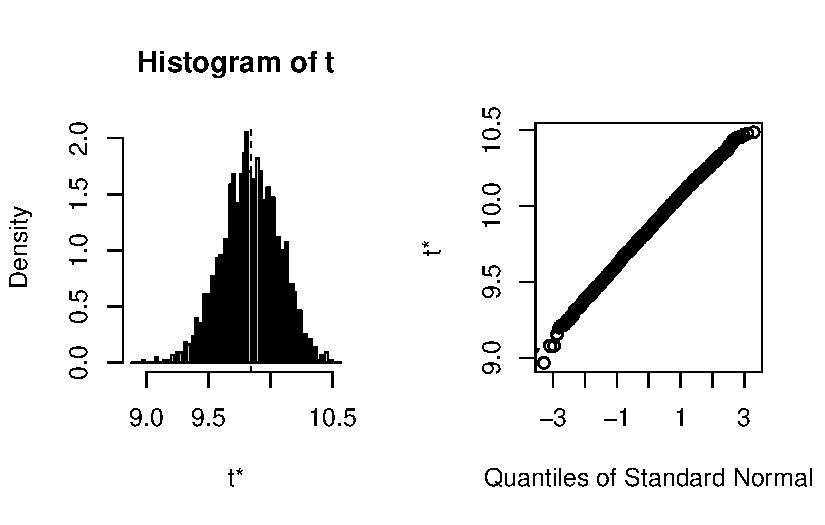
\includegraphics[keepaspectratio]{bootstrapping_methodsdav_files/figure-pdf/bootstrap-example-1.pdf}}

\begin{Shaded}
\begin{Highlighting}[]
\CommentTok{\# 5. Intervalo de confianza percentil 95\%}
\FunctionTok{boot.ci}\NormalTok{(resultados\_boot, }\AttributeTok{type =} \StringTok{"perc"}\NormalTok{)}
\end{Highlighting}
\end{Shaded}

\begin{verbatim}
BOOTSTRAP CONFIDENCE INTERVAL CALCULATIONS
Based on 2000 bootstrap replicates

CALL : 
boot.ci(boot.out = resultados_boot, type = "perc")

Intervals : 
Level     Percentile     
95%   ( 9.393, 10.272 )  
Calculations and Intervals on Original Scale
\end{verbatim}

\subsection{\texorpdfstring{\textbf{Referencias
recomendadas}}{Referencias recomendadas}}\label{referencias-recomendadas}

\begin{itemize}
\item
  Efron, B., \& Tibshirani, R. J. (1993). \emph{An Introduction to the
  Bootstrap}. Chapman \& Hall. Efron y Tibshirani (1993)
\item
  Davison, A. C., \& Hinkley, D. V. (1997). \emph{Bootstrap Methods and
  Their Application}. Cambridge University Press.
\item
  Canty, A., \& Ripley, B. (2021). boot: Bootstrap R (S-Plus) Functions.
  CRAN Package.
\end{itemize}

\phantomsection\label{refs}
\begin{CSLReferences}{1}{0}
\bibitem[\citeproctext]{ref-efron1993c}
Efron, Bradley, y Robert J. Tibshirani. 1993. \emph{An Introduction to
the Bootstrap}. Springer US.
\url{https://doi.org/10.1007/978-1-4899-4541-9}.

\end{CSLReferences}




\end{document}
